%!TEX root = da-screen.tex

Imagine that we have $n$ computers that are connected to each other with communication channels so that the network topology is a \emph{path}:
\begin{center}
    \includegraphics[page=\PIntroTopo]{figs.pdf}
\end{center}
Our task is to find a proper \emph{colouring} of the path with $3$ colours. That is, each computer has to output one of the colours, $1$, $2$, or $3$, so that neighbours have different colours:
\begin{center}
    \includegraphics[page=\PIntroCol]{figs.pdf}
\end{center}

\section{Challenges of Distributed Algorithm}

With a bird's-eye view of the entire network, colouring a path looks like a very simple task: just start from one endpoint and assign colours $1$ and $2$ alternatingly. However, in a real-world computer network we usually do not have all-powerful entities that know everything about the network and can directly tell each computer what to do.

Indeed, when we start a networked computer, it is typically only aware of itself and the communication channels that it can use. In our simple example, the endpoints of the path know that they have one neighbour:
\begin{center}
    \includegraphics[page=\PIntroDegOne]{figs.pdf}
\end{center}
All other nodes along the path just know that they have two neighbours:
\begin{center}
    \includegraphics[page=\PIntroDegTwo]{figs.pdf}
\end{center}
For example, the second node along the path looks no different from the third node, yet somehow they have to produce \emph{different} outputs.

Obviously, the nodes have to exchange \emph{messages} with each other in order to figure out a proper solution. Yet this turns out to be surprisingly difficult even in the case of just $n = 2$ nodes:
\begin{center}
    \includegraphics[page=\PIntroTwo]{figs.pdf}
\end{center}
If we have two \emph{identical} computers connected to each other with a single communication link, both computers are started simultaneously, and both of them run the same deterministic algorithm, how could they ever end up in \emph{different} states?

As we will see in Chapter~\ref{ch:intro-neg}, the answer is that it is not possible, without some additional assumptions. In practice, we could try to rely on some imperfections (e.g., the computers are seldom perfectly synchronised), but in the theory of distributed algorithms we often assume that there is some explicit way to \emph{break symmetry} between otherwise identical computers. In this chapter, we will have a brief look at two common assumption:
\begin{itemize}[noitemsep]
    \item each computer has a unique name (Section~\ref{sec:intro-pos-id}),
    \item the computers can use randomness (Section~\ref{sec:intro-pos-random}).
\end{itemize}
In subsequent chapters we will then formalise these models, and develop a theory that will help us understand precisely what kind of tasks can be solved in each case, and how fast.


\section{Colouring with Unique Identifiers}\label{sec:intro-pos-id}

There are plenty of examples of real-world networks with globally unique identifiers: public IPv4 and IPv6 addresses are globally unique identifiers of Internet hosts, devices connected to an Ethernet network have globally unique MAC addresses, mobile phones have their IMEI numbers, etc. The common theme is that the identifiers are (supposed to be) globally unique, and the numbers can be interpreted as natural numbers:
\begin{center}
    \includegraphics[page=\PIntroId]{figs.pdf}
\end{center}
With the help of unique identifiers, it is now easy to design an algorithm that colours a path. Indeed, the unique identifiers already form a colouring with a large number of colours! All that we need to do is to reduce the number of colours to $3$.

We can use the following simple strategy. In each round, all ``local maxima'' will be active, i.e., nodes with colours larger than the colours of their neighbours:
\begin{center}
    \includegraphics[page=\PIntroIdA]{figs.pdf}
\end{center}
The active nodes will then pick a new colour from the colour palette $\{1,2,3\}$, so that it does not conflict with the current colours of their neighbours. This is always possible, as each node in a path has at most $2$ neighbours, and we have $3$ colours in our colour palette:
\begin{center}
    \includegraphics[page=\PIntroIdAA]{figs.pdf}
\end{center}
Then we simply repeat the same procedure until all nodes have small colours. First find the local maxima:
\begin{center}
    \includegraphics[page=\PIntroIdB]{figs.pdf}
\end{center}
And then recolour the local maxima with colours from $\{1,2,3\}$:
\begin{center}
    \includegraphics[page=\PIntroIdBB]{figs.pdf}
\end{center}
Continuing this way we will eventually have a path that is properly coloured with colours $\{1,2,3\}$:
\begin{center}
    \includegraphics[page=\PIntroIdC]{figs.pdf}\\
    \includegraphics[page=\PIntroIdCC]{figs.pdf}\\
    \includegraphics[page=\PIntroIdD]{figs.pdf}\\
    \includegraphics[page=\PIntroIdDD]{figs.pdf}\\
    \includegraphics[page=\PIntroIdE]{figs.pdf}\\
    \includegraphics[page=\PIntroIdEE]{figs.pdf}
\end{center}
Note that we may indeed be forced to use all three colours.

So far we have sketched an algorithm idea, but we still have to show that we can actually implement this idea as a distributed algorithm. Remember that there is no central control; nobody has a bird's-eye view of the entire network. Each node is an independent computer, and all computers are running the \emph{same} algorithm. What would the algorithm look like?

Let us fix some notation. Each node maintains a variable $c$ that contains its current colour. Initially, $c$ is equal to the unique identifier of the node. Then computation proceeds as shown in Table~\ref{tab:intro-id-greedy}.

\begin{table}
    \raggedright
    \algtoprule
    \begin{descriptionb}
        \item[Repeat forever:] \mbox{}
        \begin{itemize}
            \item Send message $c$ to all neighbours.
            \item Receive messages from all neighbours. \\
                  Let $M$ be the set of messages received.
            \item If $c \notin \{1,2,3\}$ and $c > \max M$: \\
                  Let $c \gets \{1,2,3\} \setminus M$.
        \end{itemize}
    \end{descriptionb}
    \algbottomrule
    \caption{Greedy colouring of paths.}\label{tab:intro-id-greedy}
\end{table}

This shows a typical structure of a distributed algorithm: an infinite send--receive--compute loop. A computer is seen as a state machine; here $c$ is the variable that holds the current state of the computer. In this algorithm, we have three \emph{stopping states}: $c = 1$, $c = 2$, and $c = 3$. It is easy to verify that the algorithm is indeed correct in the following sense:
\begin{enumerate}
    \item In any path graph, for any assignment of unique identifiers, all computers will eventually reach a stopping state.
    \item Once a computer reaches a stopping state, it never changes its state.
\end{enumerate}
The second property is very important: each computer has to know when it is safe to announce its output and stop.

Our algorithm may look a bit strange in the sense that computers that have ``stopped'' are still sending messages. However, it is fairly straightforward to rewrite the algorithm so that you could actually turn off computers that have stopped. The basic idea is that nodes that are going to switch to a stopping state first inform their neighbours about this. Each node will memorise which of its neighbours have already stopped and what where their final colours. Implementing this idea is left as Exercise~\ref{ex:intro-stopped}, and you will later see in Exercise~\ref{ex:stopped} that this can be done for \emph{any} distributed algorithm. Hence we will play with the following simple rules:
\begin{itemize}
    \item Computers are state machines that repeatedly send messages to their neighbours, receive messages from their neighbours, and update their state.
    \item Some of the states are stopping states, and once a node reaches a stopping state, its no longer changes its state.
    \item Eventually all nodes have to reach stopping states, and these states must form a correct solution to the problem that we want to solve.
\end{itemize}



\section{Fast Colouring with Unique Identifiers}\label{sec:intro-pos-id-fast}


FIXME: Cole--Vishkin graph colouring.

\section{Colouring with Randomised Algorithms}\label{sec:intro-pos-random}

FIXME

\section{Exercises}

\begin{ex}[stopped nodes]\label{ex:intro-stopped}
    Rewrite the greedy algorithm of Table~\ref{tab:intro-id-greedy} so that stopped nodes do not need to send messages.
\end{ex}


